\chapter{Implementation}
\label{ch:implementation}

\section{System Overview}
\label{sec:system-overview}

This chapter covers the technical implementation of the proposed solution. The system consists of two components: a Unity-based mobile application used by children to practice speech exercises at different levels, and a Django-based web application used by the working SLP to create and assign exercises and monitor their patients' progress. The two systems communicate via REST API calls and JSON-formatted data, with persistent data stored in a Supabase PostgreSQL database. The purpose of this implementation is to create a functional prototype to test the project's feasibility in a real-world environment.

\begin{figure}[H]
    \centering
    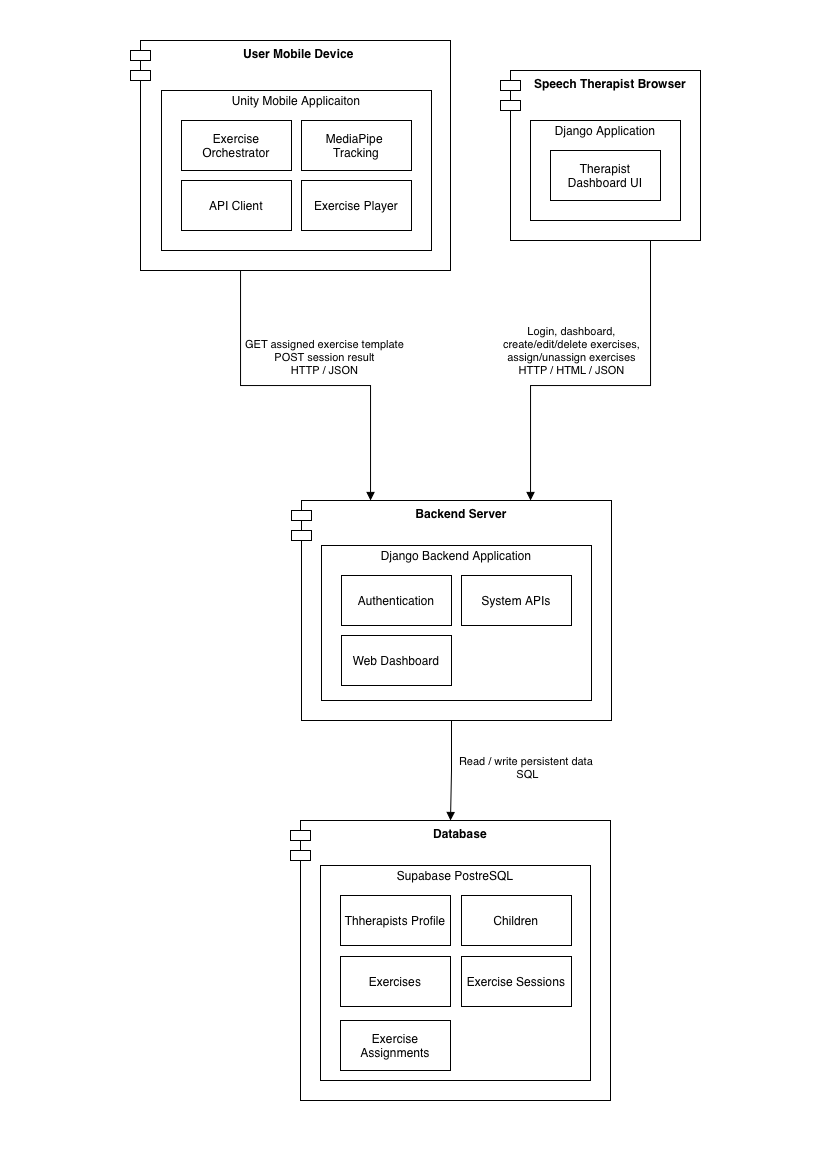
\includegraphics[height=0.78\textheight,keepaspectratio]{figures/deployment-diagram.png}
    \caption{Deployment diagram showing the mobile device, therapist browser, Django backend server, and Supabase PostgreSQL database.}
    \label{fig:deployment-diagram}
\end{figure}

\section{Technologies Used}
\label{sec:technologies-used}

Django was selected to implement the therapist dashboard and backend because it provides a well-structured web framework with extensive built-in support for API routing, templates, database modeling, and authentication with security out of the box. The system uses a decoupled architecture, with Django's web application serving as the central data management hub. System security is handled by Django's authentication framework, ensuring that only SLPs can access sensitive patient data in the dashboard. Using Django's ORM (Object-relational Mapping), the frontend is able to execute asynchronous requests and seamlessly manage database modifications. This architecture resulted in a fully functional and secure web application where therapists can view assigned children, perform CRUD operations on custom exercises, and manage and review children's assignments and session progress.

Unity was chosen as the technology behind the mobile application. Game engines like Unity are made with rapid iteration and performance in mind. This makes them a strong fit for developing on a mobile platform. Additionally, Unity offers robust UI creation tools and a feature-rich package store, further expanding its already extensive capabilities. Unity has been a staple of mobile gaming for years, with examples like \textit{Genshin Impact}, \textit{Among Us}, and \textit{Hearthstone}. It also provides a mature platform that has been used by companies such as IKEA and Volkswagen for non-gaming applications, especially when leveraging AR and VR capabilities.

For face and mouth tracking, the project integrated MediaPipe's face landmark detection pipeline into Unity. MediaPipe processes the device camera feed in real time and produces facial landmark coordinates, which are then interpreted by custom scripts. Specifically, the system captures facial positions related to the lips, jaw, and mouth contours. The custom scripts calculate distances and aspect ratios between these nodes and are able to evaluate the child's mouth position during exercises without needing additional wearable hardware.

Supabase delivers built-in user management with email/password and OAuth login, real-time data synchronization, and WebSockets that track database changes or broadcast messages across connected clients. It also offers serverless functions for custom backend logic that runs close to the user, making it a strong option for backend infrastructure. In our project, Supabase was used as a DBaaS (Database as a Service), providing a cloud-hosted, fully managed PostgreSQL database. This decision was taken based on the reliable cloud hosting of the database without the need to configure our own server. This eliminated the need for a locally hosted database server, allowing the PostgreSQL instance to be used and managed by Django's backend through its object-relational mapping system.

Communication between the Unity client and the Django backend is established via HTTP API endpoints. The Unity application sends and receives data using Unity's \texttt{UnityWebRequest} class, implemented in a dedicated C\# script called \texttt{TherapyApiClient}, exchanging data in JSON format.

\section{System Architecture}
\label{sec:system-architecture}

The system follows a client-server architecture. The Django backend acts as the server, exposing API endpoints used by both the Unity mobile client and the therapist web dashboard. The therapist dashboard communicates with Django through JavaScript \texttt{fetch} requests made from the browser. The Unity client communicates with the same backend using HTTP requests from within the application. The PostgreSQL database is fully managed by Django. All data, including exercise templates, assignments, and session results, is stored and retrieved using Django's data models.

\begin{figure}[H]
    \centering
    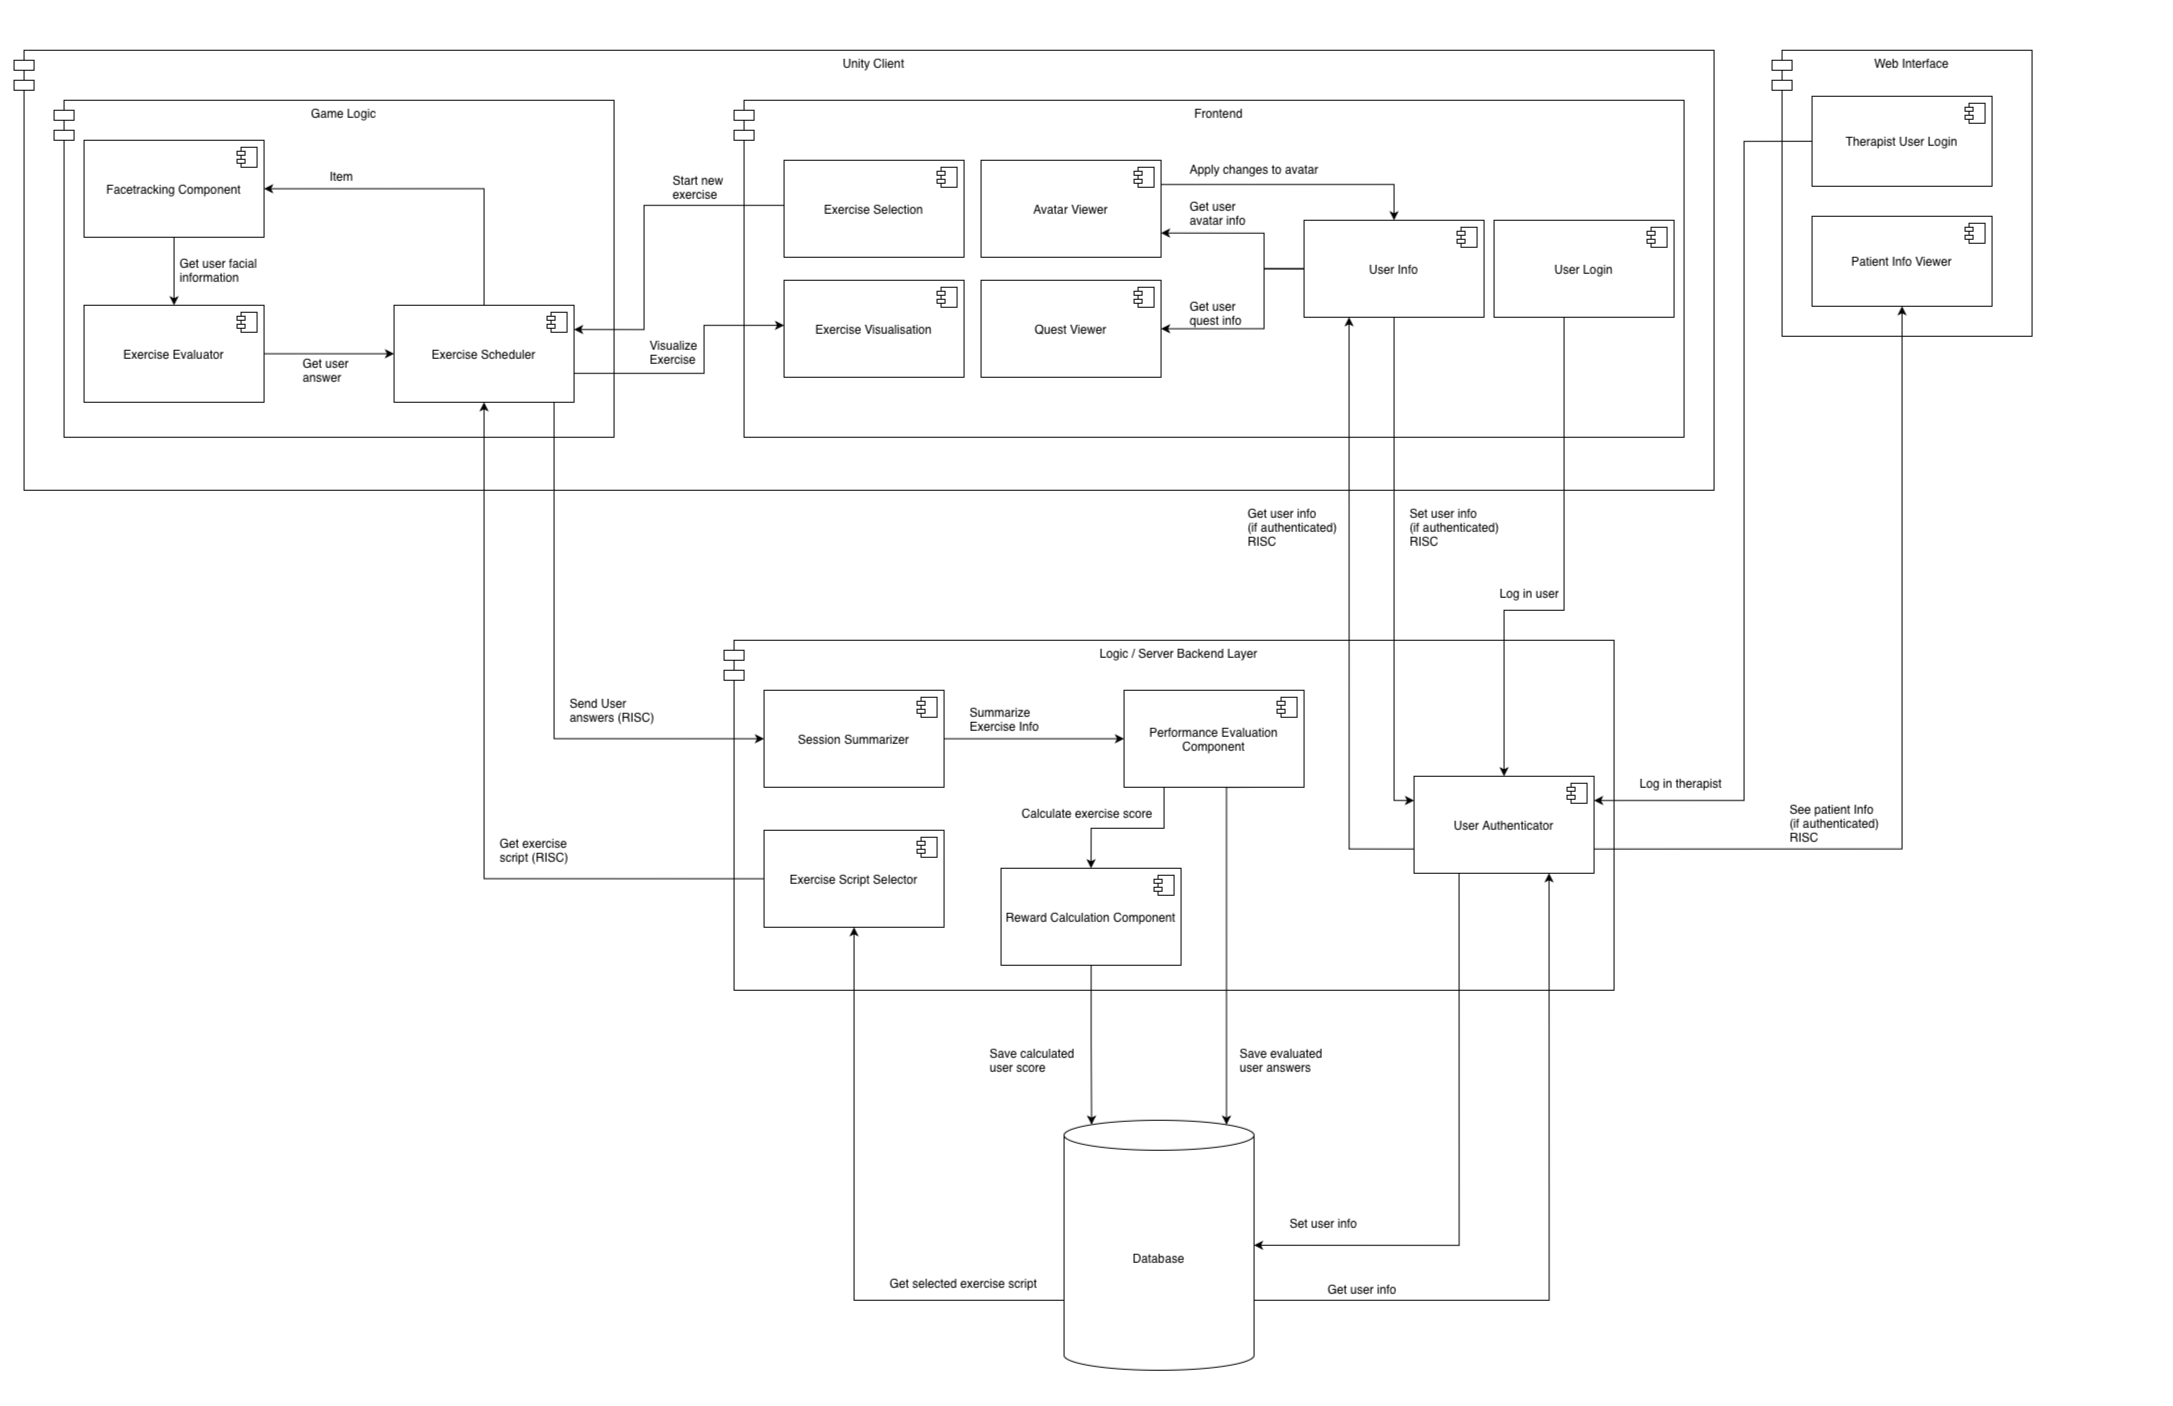
\includegraphics[width=\textwidth,height=0.72\textheight,keepaspectratio]{figures/component-architecture-diagram.png}
    \caption{Component architecture diagram showing the Unity client, web interface, backend layer, and database responsibilities.}
    \label{fig:component-architecture-diagram}
\end{figure}

The Unity mobile app is architecturally split into two main components. The game logic layer acts as a backend for the Unity client. It is responsible for sending and receiving HTTP requests from the Django backend REST API, as well as interpreting and evaluating the exercises. The frontend layer displays the avatar and quest screen, exercise selection screen, the exercises themselves, and the authentication screen.

The backend/server layer serves as the central coordination point between the Unity client, the web interface, and the database. In the architecture diagram, this layer contains components such as the session summarizer, exercise script selector, performance evaluation component, and user authenticator. These components represent the main responsibilities of the backend. The exercise script selector retrieves the correct exercise content for the child. The session summarizer receives the child's answers after an exercise session and prepares the data for storage. The performance evaluation component calculates and stores session-level information about the child's exercise performance, converting it into feedback and progress status.

The exercise content of the application is saved as a JSON template structure. This template file consists of several attributes needed for the application to render the exercise. The first and most important is the type of exercise, which determines the visual rendering of the exercise. The following attributes consist of text prompts for questions and relational mappings to correct or incorrect answers or connected words.

The web interface represents the therapist-facing part of the system, containing the therapist login and patient information viewer. In the implemented system, this corresponds to the Django therapist dashboard through which the SLP can log in, view children, create exercises, assign or unassign exercises, and inspect progress information. The web interface does not manage the database directly; instead, it communicates with the backend, which applies the appropriate business rules and updates the database.

The database is the persistent storage component. It stores information such as user data, exercise templates, selected exercise scripts, evaluated answers, calculated scores, and session history.

Overall, the architecture supports the main goal of the project: connecting therapist-managed exercise content with guided practice. The implementation covers the core parts of this architecture, namely the Unity exercise flow, the Django therapist dashboard, the backend API endpoints, and the PostgreSQL database storage. The final prototype does not implement every component with the same level of completeness as the diagram describes. For instance, reward calculation, avatar progression, and advanced performance evaluation are better understood as planned or partially implemented. Technical debt is further discussed in \Cref{ch:discussion}.

\section{Core Application Flow}
\label{sec:core-application-flow}

The typical workflow through the system proceeds as follows: a therapist logs in to the Django dashboard and is presented with a suite of tools and options that allow them to create a custom exercise or choose an existing one from the database to assign to a specific patient. Once created or chosen, it gets assigned to the selected child, and Django processes the action and stores it as an \texttt{ExerciseAssignment} record in the database.

\begin{figure}[H]
    \centering
    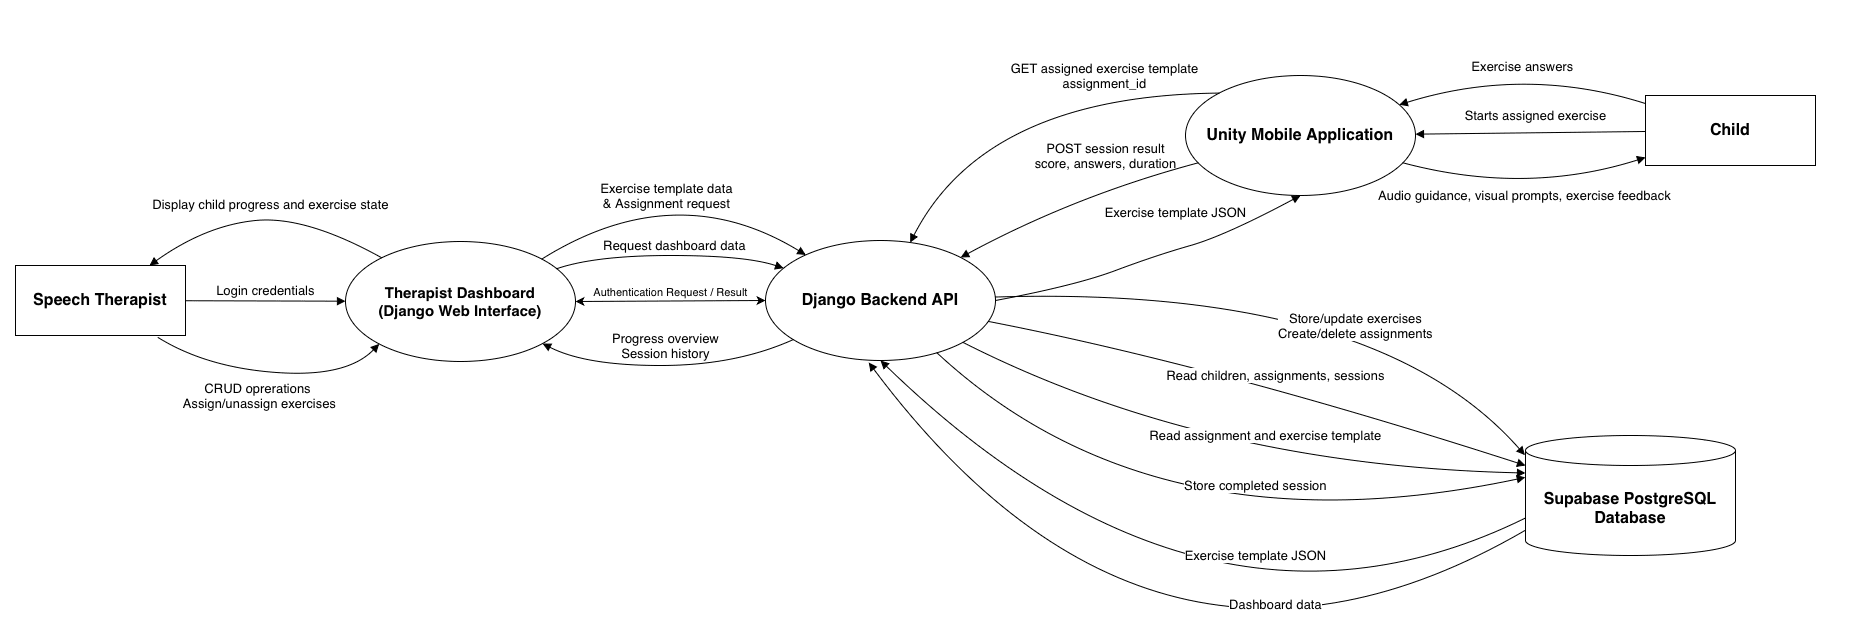
\includegraphics[width=\textwidth]{figures/dataflow-diagram.png}
    \caption{Level 1 dataflow diagram showing how exercise templates, assignments, session results, and dashboard data move through the system.}
    \label{fig:dataflow-diagram}
\end{figure}

On the Unity side, the application is assignment-driven. The Unity client holds an \texttt{assignment\_id}, which it uses to request the corresponding exercise template from the backend. When the exercise scene is started, the \texttt{Exercise\_Orchestrator} component locates the \texttt{TherapyApiClient} and calls the method responsible for fetching the assigned template. The API endpoints used by the Unity client are:

\begin{verbatim}
GET /therapy/api/assignment/<assignment_id>/template/
Returns the exercise template JSON for the given assignment.

GET /therapy/api/assignment/<assignment_id>/exercise/
Returns general assignment metadata, including the child ID,
child name, exercise title, and template JSON.

POST /therapy/api/sessions/
Uploads the result of a completed session, including score,
correct answers, total questions, duration, timestamp,
and optional event data.
\end{verbatim}

If the API request is successful, Unity parses the returned JSON and initializes the exercise. The \texttt{Exercise\_Orchestrator} then generates a queue based on the parsed exercise structure. Using this queue, the \texttt{Exercise\_Orchestrator} acts as a backend manager component, with the sole responsibility of calling high-level functions in the right sequence.

The frontend UI controls are handled by the \texttt{Exercise\_Animation\_Controller}. This separation exists to decouple backend logic from frontend logic. Once the exercise is completed, Unity sends the session result back to the Django backend through the sessions endpoint, where it is stored and made available to the therapist through the dashboard.

The application flow then comes back to the therapist dashboard. When the therapist accesses the dashboard, they are shown a detailed progress report and overview of the child. The web application shows the number of completed exercises and the number of correct answers. The therapist can review the child's performance remotely and, based on the results, formulate or adjust the structure for the patient's needs.

The Django backend serves as the communication layer between the Unity application, the therapist dashboard, and the database. It exposes API endpoints that allow the Unity client to request assigned exercises and submit completed session results. It also handles web requests from the therapist dashboard and updates the database when therapists create, edit, delete, assign, or unassign exercises.

Additionally, the project includes experimental use of MediaPipe for face and mouth tracking in Unity. This was included to explore how computer vision could support pronunciation-related exercises. However, this part of the project should be understood as experimental rather than a clinically validated assessment tool. The issues are known technical debt, discussed further in \Cref{ch:discussion}.

\section{Exercise System}
\label{sec:exercise-system}

The exercise system functions around three main components: the \texttt{Exercise\_Orchestrator}, the \texttt{Exercise\_Animation\_Controller}, and the \texttt{Milestone\_Manager}, with milestone exercises being handled separately by the latter.

\begin{figure}[H]
    \centering
    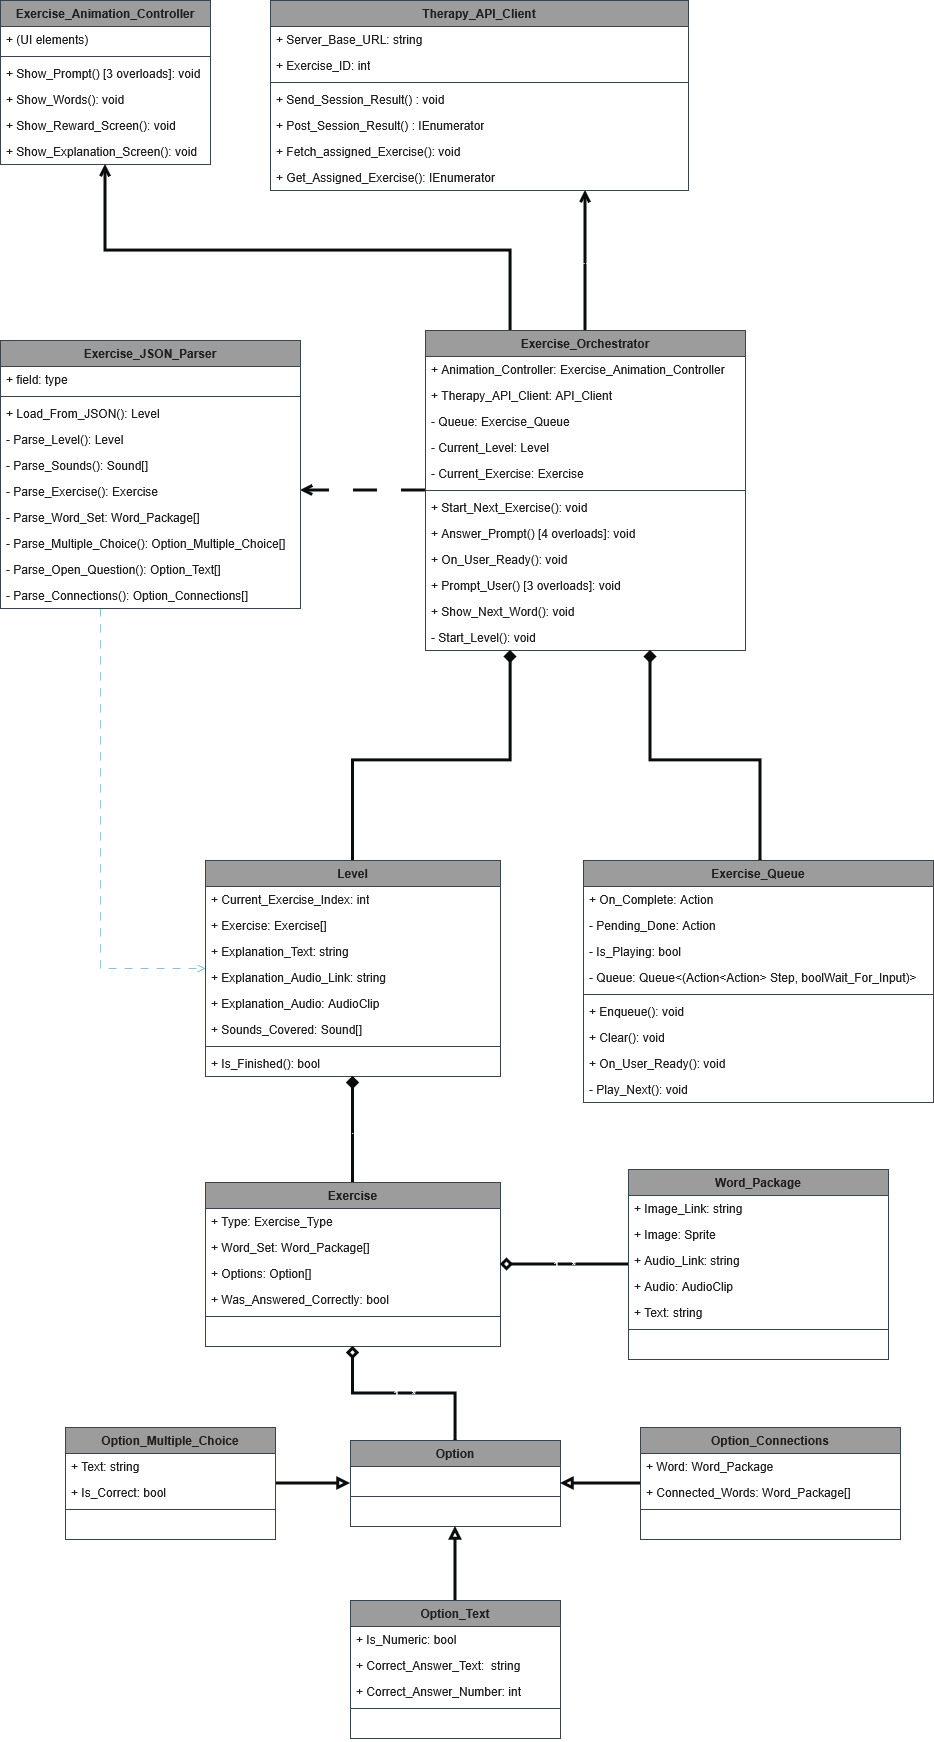
\includegraphics[height=0.82\textheight,keepaspectratio]{figures/class-diagram.png}
    \caption{Class diagram of the core Unity exercise system, including orchestration, animation, API communication, parsing, and exercise data models.}
    \label{fig:class-diagram}
\end{figure}

The \texttt{Exercise\_Orchestrator} functions around a queue. This queue is initialized with the JSON provided by the Django backend, which the \texttt{Exercise\_JSON\_Parser} component parses into a predefined level class. Using this level class, the \texttt{Exercise\_Orchestrator} is able to call high-level functions such as \texttt{Prompt\_User()} and \texttt{Show\_Next\_Word()} in the correct sequence. The queue is only advanced when \texttt{On\_User\_Ready()} is called, effectively making the flow wait for user input.

Method overloading was used throughout in order to improve readability and simplify function calls:

\begin{verbatim}
public void Prompt_User(string Question, Option_Text[] Options, Action Done)
public void Prompt_User(string Question, Option_Multiple_Choice[] Options, Action Done)
public void Prompt_User(string Question, Option_Connections[] Options, Action Done)

public void Answer_Prompt(Option_Multiple_Choice Answer)
public void Answer_Prompt(Option_Text Answer, string Answer_Text)
public void Answer_Prompt(Option_Text Answer, int Answer_Number)
public void Answer_Prompt(Option_Connections[] Answer, bool Answered_Correctly)
\end{verbatim}

The \texttt{Exercise\_Orchestrator} also handles answer evaluation. The selected option is sent by the \texttt{Exercise\_Animation\_Controller} using the \texttt{Answer\_Prompt} function. Method overloading was especially useful here since the same function name can be called from all exercise types.

The exercise system implements a set of screens, each with different responsibilities:

\begin{itemize}
    \item \textbf{Explanation Screen:} Presents a short reminder of how the sounds relevant to the exercise are produced using text, audio, and two-dimensional visualizations.
    \item \textbf{Word Showcase Screen:} Showcases the words that are to be used in the following exercise using an interactive carousel. The user sees a simulated mirror on this screen and is only allowed to continue after listening to and repeating all words shown.
    \item \textbf{Multiple Choice Screen:} Shows the user a single word and a question with a multiple-choice answer. The word is represented only by an image, but an audio recording of it can be heard when clicked.
    \item \textbf{Open Question Screen:} Shows the user a single word, a question, and an input field. The word is represented only by an image, but an audio recording of it can be heard when clicked.
    \item \textbf{Connections Screen:} Shows the user a set of words and a question. The user can connect two words by clicking on them. Each word is represented only by an image, but an audio recording of it can be heard when clicked.
    \item \textbf{Reward Screen:} Shown to the user at the end of the exercise.
\end{itemize}

The \texttt{Exercise\_Animation\_Controller} is responsible for managing all of these screens. This is done using a set of smaller components, used to produce certain effects, such as the word carousel during the word showcase screen. At the end of each exercise, a new request is sent to the Django backend with the number of correct answers.

The \texttt{Milestone\_Manager} component uses a different scene because the milestone levels are not centered around showing words to the user, but on showing text. The milestone level implements only one screen. Similar to the word showcase screen, a simulated mirror is presented to the user alongside paginated text.

At the start of the milestone level, the \texttt{FFMPEG\_Recorder} component gets triggered. As the name suggests, the \texttt{FFMPEG\_Recorder} component creates an FFmpeg process and sends each frame for video processing. Audio gets recorded separately using the integrated \texttt{Microphone.Start()} function. Since there are two separate recordings, the start of each recording is logged, and after adjusting their timing, they are combined using a separate FFmpeg process.

Videos are compressed to a few megabytes per minute. Despite this, the video recording is not currently sent to the Django backend due to Supabase's file size constraints.

\section{Results and Evaluation}
\label{sec:results-evaluation}

The success of the system depends on the execution of the core functionalities defined in the system architecture design. The solutions proposed to address the challenges identified in \Cref{ch:problem-statement} were designed as functional prototypes and tested both practically and technologically, with data flow demonstrated to an active Speech-Language Pathologist.

\subsection{Recalling Proper Exercise Execution}
\label{subsec:recalling-proper-exercise-execution}

The explanation screen was developed iteratively in the Unity exercise flow. After the core exercises were established, supporting features such as audio explanations, visual guidance, word cards, and instructions were added. The reason for those aids was that the target group may not be confident readers, thus focusing on combining sound and visual cues. This practice drill automatically starts before each level, using the sounds from the selected exercise.

This solution was evaluated by a practicing SLP, who, during a prototype demonstration, approved the chosen visuals. However, since the explanation screen has not been tested with users in the target group, further evaluation is necessary for this solution to be production-ready.

\subsection{Limited Self-Correction Without Mirror Feedback}
\label{subsec:limited-self-correction-without-mirror-feedback}

The face tracking feature mentioned in \Cref{sec:technologies-used} was treated as exploratory rather than a core deliverable. MediaPipe's face detection is part of the prototype evaluation. It shows that real-time face, mouth, and lip positions can be extracted and converted into measurable output that can later be used as a stricter method of evaluation.

The limitation of the proposed solution for this problem is that the accuracy of those measurements was not evaluated against a clinical standard, and the feature should not yet be used as a concrete assessment of valid pronunciation. However, it shows a promising direction for future development.

\subsection{Need for Therapist-Guided Personalized Exercises}
\label{subsec:need-for-therapist-guided-personalized-exercises}

The three exercise types were carefully designed to match the practice drills a patient would receive during clinical hours. The result is a JSON template with a flexible structure that can represent any new exercise an SLP would add, while remaining simple and consistent enough to be parsed and run reliably. The template allows for different exercise types, such as multiple choice, open questions, and connecting words, as well as custom correct options and audio or video recording of milestone exercises, which can be used for SLP evaluation.

The result is a modular exercise system that dynamically fetches and renders exercise content from the backend at runtime. Exercises can be created by the SLP via the Django dashboard without modifying the Unity client itself.

Additionally, the system successfully delivers the core functionality described. The prototype was presented in front of a practicing SLP who examined all the functionality and showed success in four key areas:

\begin{itemize}
    \item The SLP considered the exercise selection to be appropriate as the exercises were based on previously provided material.
    \item The SLP's positive statement that she would use such a system in her own practice supports the practical application of the concept.
    \item The SLP appreciated the distinction between the therapist-facing dashboard and the user-focused mobile application, noting that therapists assigning targeted exercises while children completed them themselves is typical of realistic clinical workflows.
    \item The SLP pointed to the mobile format as a specific practical advantage because mobile-based exercises eliminate the common issue of children forgetting or losing paper practice materials.
\end{itemize}

Although the results are positive, the system has limitations. The Unity client was originally designed as a gamified application, whereas the current prototype has shifted toward being more educational than a captivating game. Despite that, the app still has a child-friendly UI and level progression with a reward screen. Another limitation is that the current setup for the user-side flow is based on \texttt{assignment\_id} rather than user authentication. This is sufficient for a prototype workflow demonstration, but a real-world system would need a more secure identification flow.

Finally, these results should be interpreted within their appropriate scope. The evaluation was based on a single demonstration rather than repeated usage. The feedback supports the project's relevance, but it is not formal evidence of clinical effectiveness. Additional user testing involving multiple therapists, children, and caregivers should be conducted to draw stronger conclusions about the system's impact on speech practice outcomes.
